\section{Evaluation}
Throughout this section we perform experiments to answer the following research questions:
\begin{itemize}
    \item \textbf{RQ1}: How does changing $\alpha_k$ affect the performance in LightGCN?
    \item \textbf{RQ2}: How do different aggregation functions effect the performance in GCF and LightGCN?
    \item \textbf{RQ3}: How does adding ALC and BLC to LightGCN perform compared to other state of the art methods?
    \item \textbf{RQ4}: Is it beneficial to change layer combination based on the degree of the nodes?
\end{itemize}
\subsubsection{Datasets}

For our experiments, we have used 6 different datasets.
These are \textit{Yelp2020}, \textit{Amazon-Book}, \textit{Amazon-Cell-Sport}, \textit{Amazon-Cell-Electronic}, \textit{Amazon-Cloth-Electronic} and \textit{Amazon-Cloth-Sport}.
The data split is 20\% testing and 80\% training where 10\% of the training data is used as validation data.
A comparison of the datasets can be seen on \autoref{tab:dataset-comparison}.
\\
Each dataset has some applied k-core settings to it.
K-core means that all users and items with less than \textit{k} connections are removed.
This is because users and items with too few connections wont have enough data to compare to other users and items and therefore making collaborative filtering ineffective.
\\
\textbf{\textit{Amazon-Book}} is the largest dataset we have used.
It is taken from the LightGCN paper and only contains ID's for users and items \cite{lightgcn}.
LightGCN have used the 15-core setting for users and 5-core settings for items \textit{i.e.} removing users with less than 15 interactions and items with less than 5 interactions.
\\
\textbf{The \textit{Yelp2020} dataset} is a dataset we used in our pre-specialization paper to mimic a dataset used in LightGCN that we could not get access to.
This dataset uses 10-core settings for users and 5-core settings for items.
It is a subset of the full yelp2020 dataset where all entries are restaurants with one category and price attribute.
\\
\textbf{\textit{Amazon-Cell-Sport}, \textit{Amazon-Cell-Electronic}, \textit{Amazon-Cloth-Electronic} and \textit{Amazon-Cloth-Sport}} are taken from BiTGCF \cite{BiTGCF}.
These datasets contain two domains because BiTGCF builds an extension of LightGCN which utilizes a cross-domain transfer learning recommendation model \cite{BiTGCF}.
To build a cross-domain dataset first all the overlapping users were found.
Then all the users with five or more interactions were retained.
Items from each domain have both been split into training and testing before being merged.

\textit{Amazon-Cell-Sport}, \textit{Amazon-Cloth-Electronic} and \textit{Amazon-Cloth-Sport} use 5-core settings for users and 1-core settings for items.
There is an exception for \textit{Amazon-Cell-Electronic} which uses 15-core settings for users.


\paragraph{Interactions in the datasets}
As we expect there is a relation between the number of connections for each node and the performance of a convolution layer.
On \autoref{tab:dataset-item-and-user-splits} and \autoref{tab:node-degrees-cell-sport-electronic} each degree range of users and items can be seen as well as what amount of users and items each dataset have of each degree range.
Users in \textit{Amazon-Book} have an average node degree of 45.22 and items have an average node degree of 25.99 connections, which makes it the dataset with the highest average node degree compared to the other datasets.
For Yelp2020 the average node degree is 19.04 for users and 23.31 for items.
The other four amazon datasets have in common that the average node degree for items is small.
Users in \textit{Amazon-Cell-Sport} have an average node degree of 17.07 and items have an average node degree of 2.58.
\textit{Amazon-Cell-Electronic} has an average node degree of 42.22 for users and an average node degree 2.73 for items.
\textit{Amazon-Cloth-Electronic} has an average node degree of 19.04 for users and an average node degree of 3.12 for items.
\textit{Amazon-Cloth-Sport} has an average node degree of 16.72 for users and an average node degree of 2.49 for items.
\\
\\
These core-settings was chosen based on what the datasets in Bit-GCF and LightGCN used. 
This way we felt it was more fair to compare our method to the dataset that the other state of the art methods utilized.


\begin{table*}[]
    \scriptsize
    \begin{tabular}{|l|l|l|l|l|l|l|l|l|l|l|l|l|}
        \hline
                & \multicolumn{4}{c|}{Yelp2020} & \multicolumn{4}{c|}{Amazon-Cell-Sport} & \multicolumn{4}{c|}{Amazon-Book}                                                                                                                                                     \\ \hline
        Degree   & \multicolumn{2}{c|}{Users}    & \multicolumn{2}{c|}{Items}             & \multicolumn{2}{c|}{Users}       & \multicolumn{2}{c|}{Items} & \multicolumn{2}{c|}{Users} & \multicolumn{2}{c|}{Items}                                                              \\ \hline
        1-5     & 0                             & 0 \%                                   & 5185                             & 26.02 \%                   & 0                          & 0 \%                       & 30152 & 91.31 \%     & 0     & 0 \%     & 4393  & 4.79  \% \\ \hline
        6-10    & 7298                          & 29.92 \%                               & 4652                             & 23.34 \%                   & 1190                       & 23.80 \%                   & 1677  & 5.07 \%      & 0     & 0 \%     & 20562 & 22.44 \% \\ \hline
        11-15   & 7175                          & 29.42 \%                               & 2505                             & 12.57 \%                   & 1890                       & 37.81 \%                   & 565   & 1.71 \%      & 0     & 0 \%     & 21561 & 23.53 \% \\ \hline
        16-20   & 3862                          & 15.83 \%                               & 1622                             & 8.14 \%                    & 936                        & 18.72 \%                   & 270   & 0.817 \%     & 17098 & 32.47 \% & 12092 & 13.20 \% \\ \hline
        21-25   & 1742                          & 7.14 \%                                & 1135                             & 5.69 \%                    & 396                        & 7.92 \%                    & 137   & 0.41 \%      & 8234  & 15.64 \% & 7638  & 8.33 \%  \\ \hline
        26-30   & 1160                          & 4.75 \%                                & 814                              & 4.08 \%                    & 211                        & 4.22 \%                    & 78    & 0.23 \%      & 5257  & 9.98 \%  & 5092  & 5.55 \%  \\ \hline
        31-35   & 749                           & 3.07 \%                                & 624                              & 3.13 \%                    & 115                        & 2.30 \%                    & 44    & 0.133 \%     & 3722  & 7.07 \%  & 3791  & 4.13 \%  \\ \hline
        36-40   & 664                           & 2.72 \%                                & 487                              & 2.44 \%                    & 78                         & 1.56 \%                    & 27    & 0.081 \%     & 3154  & 5.99 \%  & 2891  & 3.15 \%  \\ \hline
        41-45   & 380                           & 1.55 \%                                & 398                              & 1.99 \%                    & 46                         & 0.92 \%                    & 19    & 0.057 \%     & 2029  & 3.85 \%  & 2301  & 2.51 \%  \\ \hline
        46-50   & 243                           & 0.99 \%                                & 323                              & 1.62 \%                    & 31                         & 0.62 \%                    & 14    & 0.042 \%     & 1591  & 3.02 \%  & 1775  & 1.93 \%  \\ \hline
        51-60   & 409                           & 1.67 \%                                & 475                              & 2.38 \%                    & 36                         & 0.72 \%                    & 13    & 0.039 \%     & 2581  & 4.90 \%  & 2407  & 2.62 \%  \\ \hline
        61-70   & 200                           & 0.82 \%                                & 316                              & 1.58 \%                    & 19                         & 0.38 \%                    & 5     & 0.015 \%     & 1664  & 3.16 \%  & 1662  & 1.81 \%  \\ \hline
        71-80   & 126                           & 0.51 \%                                & 271                              & 1.36 \%                    & 13                         & 0.26 \%                    & 6     & 0.018 \%     & 1379  & 2.61 \%  & 1183  & 1.29 \%  \\ \hline
        81-90   & 102                           & 0.41 \%                                & 199                              & 0.99 \%                    & 5                          & 0.10 \%                    & 4     & 0.012     \% & 954   & 1.81 \%  & 883   & 0.96 \%  \\ \hline
        91-100  & 71                            & 0.29 \%                                & 145                              & 0.72 \%                    & 6                          & 0.12 \%                    & 0     & 0 \%         & 745   & 1.41 \%  & 619   & 0.67 \%  \\ \hline
        101-150 & 127                           & 0.52 \%                                & 434                              & 2.17 \%                    & 23                         & 0.46 \%                    & 6     & 0.018 \%     & 2120  & 4.02 \%  & 1528  & 1.66 \%  \\ \hline
        151-200 & 52                            & 0.21 \%                                & 179                              & 0.89 \%                    & 2                          & 0.04 \%                    & 1     & 0.003     \% & 892   & 1.69 \%  & 553   & 0.60 \%  \\ \hline
        201-250 & 17                            & 0.06 \%                                & 64                               & 0.32 \%                    & 0                          & 0    \%                    & 0     & 0     \%     & 469   & 0.89 \%  & 251   & 0.27 \%  \\ \hline
        251-300 & 1                             & 0.004 \%                               & 36                               & 0.18 \%                    & 0                          & 0    \%                    & 0     & 0     \%     & 254   & 0.48 \%  & 146   & 0.15 \%  \\ \hline
        300+    & 7                             & 0.028 \%                               & 61                               & 0.30 \%                    & 1                          & 0.02 \%                    & 0     & 0  \%        & 500   & 0.94 \%  & 271   & 0.29 \%  \\ \hline
        Avg con & \multicolumn{2}{l|}{19.04}    & \multicolumn{2}{l|}{23.31}             & \multicolumn{2}{l|}{17.07}       & \multicolumn{2}{l|}{2.58}  & \multicolumn{2}{l|}{45.22} & \multicolumn{2}{l|}{25.99}                                                              \\ \hline
    \end{tabular}
    \caption{Amount of nodes within a certain node degree for Amazon-Cell-Sport, Amazon-Book and Yelp2020. The Avg connection shows how many connections each user or item have on average}
    \label{tab:dataset-item-and-user-splits}
\end{table*}

\begin{table*}[]
    \scriptsize
    \centering
    \begin{tabular}{|l|l|l|l|l|l|l|l|l|l|l|l|l|}
        \hline
                & \multicolumn{4}{c|}{Amazon-Cell-Electronic} & \multicolumn{4}{c|}{Amazon-Cloth-Electronic} & \multicolumn{4}{c|}{Amazon-Cloth-Sport}                                                                                                                                        \\ \hline
        Degree   & \multicolumn{2}{c|}{Users}                  & \multicolumn{2}{c|}{Items}                   & \multicolumn{2}{c|}{Users}              & \multicolumn{2}{c|}{Items} & \multicolumn{2}{c|}{Users} & \multicolumn{2}{c|}{Items}                                                 \\ \hline
        1-5     & \multicolumn{1}{r|}{0}                      & \multicolumn{1}{r|}{0.0 \%}                     & \multicolumn{1}{r|}{46183}              & \multicolumn{1}{r|}{89.94\%} & \multicolumn{1}{r|}{0}     & \multicolumn{1}{r|}{0.0 \%}   & 85169 & 88.81 \% & 0    & 0.0 \%   & 61217 & 91.85 \%\\ \hline
        6-10    & \multicolumn{1}{r|}{0}                      & \multicolumn{1}{r|}{0.0 \%}                     & \multicolumn{1}{r|}{3072}               & \multicolumn{1}{r|}{5.982\%} & \multicolumn{1}{r|}{3345}  & \multicolumn{1}{r|}{21.22 \%} & 6505  & 6.783 \% & 2331 & 23.479 \%& 3603  & 5.406 \%\\ \hline
        11-15   & \multicolumn{1}{r|}{0}                      & \multicolumn{1}{r|}{0.0 \%}                     & \multicolumn{1}{r|}{990}                & \multicolumn{1}{r|}{1.928\%} & \multicolumn{1}{r|}{5625}  & \multicolumn{1}{r|}{35.68 \%} & 1944  & 2.027 \% & 3675 & 37.016 \%& 979   & 1.468 \%\\ \hline
        16-20   & 538                                         & 16.180 \%                                      & 477                                     & 0.928 \%                     & 2957                       & 18.76 \%                     & 862   & 0.898 \% & 1853 & 18.664 \%& 364   & 0.546 \%\\ \hline
        21-25   & 685                                         & 20.601 \%                                      & 204                                     & 0.397 \%                     & 1358                       & 8.616 \%                     & 429   & 0.447 \% & 916  & 9.226 \% & 168   & 0.252 \%\\ \hline
        26-30   & 477                                         & 14.345 \%                                      & 128                                     & 0.249 \%                     & 774                        & 4.910 \%                     & 243   & 0.253 \%& 443  & 4.462 \% & 110   & 0.165 \%\\ \hline
        31-35   & 334                                         & 10.045 \%                                      & 63                                      & 0.122 \%                     & 458                        & 2.905 \%                     & 170   & 0.177 \%& 244  & 2.457 \% & 56    & 0.084 \%\\ \hline
        36-40   & 250                                         & 7.518 \%                                       & 61                                      & 0.118 \%                     & 295                        & 1.871 \%                     & 131   & 0.136 \%& 149  & 1.500 \% & 53    & 0.079 \%\\ \hline
        41-45   & 177                                         & 5.323 \%                                       & 42                                      & 0.081 \%                     & 208                        & 1.319 \%                     & 97    & 0.101 \%& 95   & 0.956 \% & 32    & 0.048 \%\\ \hline
        46-50   & 146                                         & 4.390 \%                                       & 29                                      & 0.056 \%                     & 157                        & 0.996 \%                     & 63    & 0.065 \%& 64   & 0.644 \% & 17    & 0.025 \%\\ \hline
        51-60   & 194                                         & 5.834 \%                                       & 40                                      & 0.077 \%                     & 186                        & 1.180 \%                     & 67    & 0.069 \%& 62   & 0.624 \% & 23    & 0.034 \%\\ \hline
        61-70   & 144                                         & 4.330 \%                                       & 16                                      & 0.031 \%                     & 107                        & 0.678 \%                     & 51    & 0.053 \%& 37   & 0.372 \% & 6     & 0.009 \%\\ \hline
        71-80   & 98                                          & 2.947 \%                                       & 12                                      & 0.023 \%                     & 83                         & 0.526 \%                     & 41    & 0.042 \%& 16   & 0.161 \% & 4     & 0.006 \%\\ \hline
        81-90   & 60                                          & 1.804 \%                                       & 13                                      & 0.025 \%                     & 48                         & 0.304 \%                     & 29    & 0.030 \%& 17   & 0.171 \% & 5     & 0.007 \%\\ \hline
        91-100  & 44                                          & 1.323 \%                                       & 7                                       & 0.013 \%                     & 37                         & 0.234 \%                     & 15    & 0.015 \%& 11   & 0.110 \% & 2     & 0.003 \%\\ \hline
        101-150 & 100                                         & 3.007 \%                                       & 8                                       & 0.015 \%                     & 68                         & 0.431 \%                     & 45    & 0.046 \%& 10   & 0.100 \% & 5     & 0.007 \%\\ \hline
        151-200 & 41                                          & 1.233 \%                                       & 2                                       & 0.003 \%                     & 37                         & 0.234 \%                     & 14    & 0.014 \%& 4    & 0.040 \% & 0     & 0.0 \%\\ \hline
        201-250 & 16                                          & 0.481 \%                                       & 0                                       & 0.0 \%                       & 12                         & 0.076 \%                     & 11    & 0.011 \%& 0    & 0.0 \%   & 0     & 0.0 \%   \\ \hline
        251-300 & 10                                          & 0.300 \%                                       & 0                                       & 0.0 \%                       & 2                          & 0.012 \%                     & 2     & 0.002 \%& 1    & 0.0100 \% & 0     & 0.0 \%  \\ \hline
        300+    & 11                                          & 0.330 \%                                       & 1                                       & 0.0019 \%                    & 4                          & 0.025 \%                     & 7     & 0.007 \%& 0    & 0.0 \%    & 0     & 0.0 \%  \\ \hline
        Avg con & \multicolumn{2}{l|}{42.22}                  & \multicolumn{2}{l|}{2.73}                    & \multicolumn{2}{l|}{19.04}              & \multicolumn{2}{l|}{3.12}  & \multicolumn{2}{l|}{16.72} & \multicolumn{2}{l|}{2.49}                                                  \\ \hline
    \end{tabular}
    \caption{Amount of nodes within a certain node degree for Amazon-Cell-Electronic, Amazon-Cloth-Electronic and Amazon-Cloth-Sport. The Avg connection shows how many connections each user or item have in average}
    \label{tab:node-degrees-cell-sport-electronic}
\end{table*}

\begin{table*}[h!]
    \scriptsize
    \centering
    \begin{tabular}{|l|l|l|l|l|l|}
        \hline
                                & Users  & Items   & Items/users ratio & Interactions & Sparsity  \\ \hline
        Amazon-Book             & 52,643 & 91,599  & 1.74              & 2,984,108    & 99.9381\% \\ \hline
        Yelp2020                & 24,384 & 20,091  & 0.824             & 594,196      & 99.8787\% \\ \hline
        Amazon-Cell-Sport       & 4,998  & 36,719  & 7.347             & 103,000      & 99.9438\% \\ \hline
        Amazon-Cell-Electronic  & 3,325  & 57,925  & 17.42             & 172,611      & 99.9103\% \\ \hline
        Amazon-Cloth-Electronic & 15,761 & 105,174 & 6.673             & 363,474      & 99,9780\% \\ \hline
        Amazon-Cloth-Sport      & 9,928  & 73,613  & 7.414             & 200,297      & 99,9726\% \\ \hline
    \end{tabular}
    \caption{Comparisons on the datasets}
    \label{tab:dataset-comparison}
\end{table*}


\subsection{Experimental Settings}

In this subsection is the datasets and the settings that has been used for the experiments outlined.

\subsubsection{Datasets}

For our experiments, we have used 6 different datasets.
These are \textit{Yelp2020}, \textit{Amazon-Book}, \textit{Amazon-Cell-Sport}, \textit{Amazon-Cell-Electronic}, \textit{Amazon-Cloth-Electronic} and \textit{Amazon-Cloth-Sport}.
The data split is 20\% testing and 80\% training where 10\% of the training data is used as validation data.
A comparison of the datasets can be seen on \autoref{tab:dataset-comparison}.
\\
Each dataset has some applied k-core settings to it.
K-core means that all users and items with less than \textit{k} connections are removed.
This is because users and items with too few connections wont have enough data to compare to other users and items and therefore making collaborative filtering ineffective.
\\
\textbf{\textit{Amazon-Book}} is the largest dataset we have used.
It is taken from the LightGCN paper and only contains ID's for users and items \cite{lightgcn}.
LightGCN have used the 15-core setting for users and 5-core settings for items \textit{i.e.} removing users with less than 15 interactions and items with less than 5 interactions.
\\
\textbf{The \textit{Yelp2020} dataset} is a dataset we used in our pre-specialization paper to mimic a dataset used in LightGCN that we could not get access to.
This dataset uses 10-core settings for users and 5-core settings for items.
It is a subset of the full yelp2020 dataset where all entries are restaurants with one category and price attribute.
\\
\textbf{\textit{Amazon-Cell-Sport}, \textit{Amazon-Cell-Electronic}, \textit{Amazon-Cloth-Electronic} and \textit{Amazon-Cloth-Sport}} are taken from BiTGCF \cite{BiTGCF}.
These datasets contain two domains because BiTGCF builds an extension of LightGCN which utilizes a cross-domain transfer learning recommendation model \cite{BiTGCF}.
To build a cross-domain dataset first all the overlapping users were found.
Then all the users with five or more interactions were retained.
Items from each domain have both been split into training and testing before being merged.

\textit{Amazon-Cell-Sport}, \textit{Amazon-Cloth-Electronic} and \textit{Amazon-Cloth-Sport} use 5-core settings for users and 1-core settings for items.
There is an exception for \textit{Amazon-Cell-Electronic} which uses 15-core settings for users.


\paragraph{Interactions in the datasets}
As we expect there is a relation between the number of connections for each node and the performance of a convolution layer.
On \autoref{tab:dataset-item-and-user-splits} and \autoref{tab:node-degrees-cell-sport-electronic} each degree range of users and items can be seen as well as what amount of users and items each dataset have of each degree range.
Users in \textit{Amazon-Book} have an average node degree of 45.22 and items have an average node degree of 25.99 connections, which makes it the dataset with the highest average node degree compared to the other datasets.
For Yelp2020 the average node degree is 19.04 for users and 23.31 for items.
The other four amazon datasets have in common that the average node degree for items is small.
Users in \textit{Amazon-Cell-Sport} have an average node degree of 17.07 and items have an average node degree of 2.58.
\textit{Amazon-Cell-Electronic} has an average node degree of 42.22 for users and an average node degree 2.73 for items.
\textit{Amazon-Cloth-Electronic} has an average node degree of 19.04 for users and an average node degree of 3.12 for items.
\textit{Amazon-Cloth-Sport} has an average node degree of 16.72 for users and an average node degree of 2.49 for items.
\\
\\
These core-settings was chosen based on what the datasets in Bit-GCF and LightGCN used. 
This way we felt it was more fair to compare our method to the dataset that the other state of the art methods utilized.


\begin{table*}[]
    \scriptsize
    \begin{tabular}{|l|l|l|l|l|l|l|l|l|l|l|l|l|}
        \hline
                & \multicolumn{4}{c|}{Yelp2020} & \multicolumn{4}{c|}{Amazon-Cell-Sport} & \multicolumn{4}{c|}{Amazon-Book}                                                                                                                                                     \\ \hline
        Degree   & \multicolumn{2}{c|}{Users}    & \multicolumn{2}{c|}{Items}             & \multicolumn{2}{c|}{Users}       & \multicolumn{2}{c|}{Items} & \multicolumn{2}{c|}{Users} & \multicolumn{2}{c|}{Items}                                                              \\ \hline
        1-5     & 0                             & 0 \%                                   & 5185                             & 26.02 \%                   & 0                          & 0 \%                       & 30152 & 91.31 \%     & 0     & 0 \%     & 4393  & 4.79  \% \\ \hline
        6-10    & 7298                          & 29.92 \%                               & 4652                             & 23.34 \%                   & 1190                       & 23.80 \%                   & 1677  & 5.07 \%      & 0     & 0 \%     & 20562 & 22.44 \% \\ \hline
        11-15   & 7175                          & 29.42 \%                               & 2505                             & 12.57 \%                   & 1890                       & 37.81 \%                   & 565   & 1.71 \%      & 0     & 0 \%     & 21561 & 23.53 \% \\ \hline
        16-20   & 3862                          & 15.83 \%                               & 1622                             & 8.14 \%                    & 936                        & 18.72 \%                   & 270   & 0.817 \%     & 17098 & 32.47 \% & 12092 & 13.20 \% \\ \hline
        21-25   & 1742                          & 7.14 \%                                & 1135                             & 5.69 \%                    & 396                        & 7.92 \%                    & 137   & 0.41 \%      & 8234  & 15.64 \% & 7638  & 8.33 \%  \\ \hline
        26-30   & 1160                          & 4.75 \%                                & 814                              & 4.08 \%                    & 211                        & 4.22 \%                    & 78    & 0.23 \%      & 5257  & 9.98 \%  & 5092  & 5.55 \%  \\ \hline
        31-35   & 749                           & 3.07 \%                                & 624                              & 3.13 \%                    & 115                        & 2.30 \%                    & 44    & 0.133 \%     & 3722  & 7.07 \%  & 3791  & 4.13 \%  \\ \hline
        36-40   & 664                           & 2.72 \%                                & 487                              & 2.44 \%                    & 78                         & 1.56 \%                    & 27    & 0.081 \%     & 3154  & 5.99 \%  & 2891  & 3.15 \%  \\ \hline
        41-45   & 380                           & 1.55 \%                                & 398                              & 1.99 \%                    & 46                         & 0.92 \%                    & 19    & 0.057 \%     & 2029  & 3.85 \%  & 2301  & 2.51 \%  \\ \hline
        46-50   & 243                           & 0.99 \%                                & 323                              & 1.62 \%                    & 31                         & 0.62 \%                    & 14    & 0.042 \%     & 1591  & 3.02 \%  & 1775  & 1.93 \%  \\ \hline
        51-60   & 409                           & 1.67 \%                                & 475                              & 2.38 \%                    & 36                         & 0.72 \%                    & 13    & 0.039 \%     & 2581  & 4.90 \%  & 2407  & 2.62 \%  \\ \hline
        61-70   & 200                           & 0.82 \%                                & 316                              & 1.58 \%                    & 19                         & 0.38 \%                    & 5     & 0.015 \%     & 1664  & 3.16 \%  & 1662  & 1.81 \%  \\ \hline
        71-80   & 126                           & 0.51 \%                                & 271                              & 1.36 \%                    & 13                         & 0.26 \%                    & 6     & 0.018 \%     & 1379  & 2.61 \%  & 1183  & 1.29 \%  \\ \hline
        81-90   & 102                           & 0.41 \%                                & 199                              & 0.99 \%                    & 5                          & 0.10 \%                    & 4     & 0.012     \% & 954   & 1.81 \%  & 883   & 0.96 \%  \\ \hline
        91-100  & 71                            & 0.29 \%                                & 145                              & 0.72 \%                    & 6                          & 0.12 \%                    & 0     & 0 \%         & 745   & 1.41 \%  & 619   & 0.67 \%  \\ \hline
        101-150 & 127                           & 0.52 \%                                & 434                              & 2.17 \%                    & 23                         & 0.46 \%                    & 6     & 0.018 \%     & 2120  & 4.02 \%  & 1528  & 1.66 \%  \\ \hline
        151-200 & 52                            & 0.21 \%                                & 179                              & 0.89 \%                    & 2                          & 0.04 \%                    & 1     & 0.003     \% & 892   & 1.69 \%  & 553   & 0.60 \%  \\ \hline
        201-250 & 17                            & 0.06 \%                                & 64                               & 0.32 \%                    & 0                          & 0    \%                    & 0     & 0     \%     & 469   & 0.89 \%  & 251   & 0.27 \%  \\ \hline
        251-300 & 1                             & 0.004 \%                               & 36                               & 0.18 \%                    & 0                          & 0    \%                    & 0     & 0     \%     & 254   & 0.48 \%  & 146   & 0.15 \%  \\ \hline
        300+    & 7                             & 0.028 \%                               & 61                               & 0.30 \%                    & 1                          & 0.02 \%                    & 0     & 0  \%        & 500   & 0.94 \%  & 271   & 0.29 \%  \\ \hline
        Avg con & \multicolumn{2}{l|}{19.04}    & \multicolumn{2}{l|}{23.31}             & \multicolumn{2}{l|}{17.07}       & \multicolumn{2}{l|}{2.58}  & \multicolumn{2}{l|}{45.22} & \multicolumn{2}{l|}{25.99}                                                              \\ \hline
    \end{tabular}
    \caption{Amount of nodes within a certain node degree for Amazon-Cell-Sport, Amazon-Book and Yelp2020. The Avg connection shows how many connections each user or item have on average}
    \label{tab:dataset-item-and-user-splits}
\end{table*}

\begin{table*}[]
    \scriptsize
    \centering
    \begin{tabular}{|l|l|l|l|l|l|l|l|l|l|l|l|l|}
        \hline
                & \multicolumn{4}{c|}{Amazon-Cell-Electronic} & \multicolumn{4}{c|}{Amazon-Cloth-Electronic} & \multicolumn{4}{c|}{Amazon-Cloth-Sport}                                                                                                                                        \\ \hline
        Degree   & \multicolumn{2}{c|}{Users}                  & \multicolumn{2}{c|}{Items}                   & \multicolumn{2}{c|}{Users}              & \multicolumn{2}{c|}{Items} & \multicolumn{2}{c|}{Users} & \multicolumn{2}{c|}{Items}                                                 \\ \hline
        1-5     & \multicolumn{1}{r|}{0}                      & \multicolumn{1}{r|}{0.0 \%}                     & \multicolumn{1}{r|}{46183}              & \multicolumn{1}{r|}{89.94\%} & \multicolumn{1}{r|}{0}     & \multicolumn{1}{r|}{0.0 \%}   & 85169 & 88.81 \% & 0    & 0.0 \%   & 61217 & 91.85 \%\\ \hline
        6-10    & \multicolumn{1}{r|}{0}                      & \multicolumn{1}{r|}{0.0 \%}                     & \multicolumn{1}{r|}{3072}               & \multicolumn{1}{r|}{5.982\%} & \multicolumn{1}{r|}{3345}  & \multicolumn{1}{r|}{21.22 \%} & 6505  & 6.783 \% & 2331 & 23.479 \%& 3603  & 5.406 \%\\ \hline
        11-15   & \multicolumn{1}{r|}{0}                      & \multicolumn{1}{r|}{0.0 \%}                     & \multicolumn{1}{r|}{990}                & \multicolumn{1}{r|}{1.928\%} & \multicolumn{1}{r|}{5625}  & \multicolumn{1}{r|}{35.68 \%} & 1944  & 2.027 \% & 3675 & 37.016 \%& 979   & 1.468 \%\\ \hline
        16-20   & 538                                         & 16.180 \%                                      & 477                                     & 0.928 \%                     & 2957                       & 18.76 \%                     & 862   & 0.898 \% & 1853 & 18.664 \%& 364   & 0.546 \%\\ \hline
        21-25   & 685                                         & 20.601 \%                                      & 204                                     & 0.397 \%                     & 1358                       & 8.616 \%                     & 429   & 0.447 \% & 916  & 9.226 \% & 168   & 0.252 \%\\ \hline
        26-30   & 477                                         & 14.345 \%                                      & 128                                     & 0.249 \%                     & 774                        & 4.910 \%                     & 243   & 0.253 \%& 443  & 4.462 \% & 110   & 0.165 \%\\ \hline
        31-35   & 334                                         & 10.045 \%                                      & 63                                      & 0.122 \%                     & 458                        & 2.905 \%                     & 170   & 0.177 \%& 244  & 2.457 \% & 56    & 0.084 \%\\ \hline
        36-40   & 250                                         & 7.518 \%                                       & 61                                      & 0.118 \%                     & 295                        & 1.871 \%                     & 131   & 0.136 \%& 149  & 1.500 \% & 53    & 0.079 \%\\ \hline
        41-45   & 177                                         & 5.323 \%                                       & 42                                      & 0.081 \%                     & 208                        & 1.319 \%                     & 97    & 0.101 \%& 95   & 0.956 \% & 32    & 0.048 \%\\ \hline
        46-50   & 146                                         & 4.390 \%                                       & 29                                      & 0.056 \%                     & 157                        & 0.996 \%                     & 63    & 0.065 \%& 64   & 0.644 \% & 17    & 0.025 \%\\ \hline
        51-60   & 194                                         & 5.834 \%                                       & 40                                      & 0.077 \%                     & 186                        & 1.180 \%                     & 67    & 0.069 \%& 62   & 0.624 \% & 23    & 0.034 \%\\ \hline
        61-70   & 144                                         & 4.330 \%                                       & 16                                      & 0.031 \%                     & 107                        & 0.678 \%                     & 51    & 0.053 \%& 37   & 0.372 \% & 6     & 0.009 \%\\ \hline
        71-80   & 98                                          & 2.947 \%                                       & 12                                      & 0.023 \%                     & 83                         & 0.526 \%                     & 41    & 0.042 \%& 16   & 0.161 \% & 4     & 0.006 \%\\ \hline
        81-90   & 60                                          & 1.804 \%                                       & 13                                      & 0.025 \%                     & 48                         & 0.304 \%                     & 29    & 0.030 \%& 17   & 0.171 \% & 5     & 0.007 \%\\ \hline
        91-100  & 44                                          & 1.323 \%                                       & 7                                       & 0.013 \%                     & 37                         & 0.234 \%                     & 15    & 0.015 \%& 11   & 0.110 \% & 2     & 0.003 \%\\ \hline
        101-150 & 100                                         & 3.007 \%                                       & 8                                       & 0.015 \%                     & 68                         & 0.431 \%                     & 45    & 0.046 \%& 10   & 0.100 \% & 5     & 0.007 \%\\ \hline
        151-200 & 41                                          & 1.233 \%                                       & 2                                       & 0.003 \%                     & 37                         & 0.234 \%                     & 14    & 0.014 \%& 4    & 0.040 \% & 0     & 0.0 \%\\ \hline
        201-250 & 16                                          & 0.481 \%                                       & 0                                       & 0.0 \%                       & 12                         & 0.076 \%                     & 11    & 0.011 \%& 0    & 0.0 \%   & 0     & 0.0 \%   \\ \hline
        251-300 & 10                                          & 0.300 \%                                       & 0                                       & 0.0 \%                       & 2                          & 0.012 \%                     & 2     & 0.002 \%& 1    & 0.0100 \% & 0     & 0.0 \%  \\ \hline
        300+    & 11                                          & 0.330 \%                                       & 1                                       & 0.0019 \%                    & 4                          & 0.025 \%                     & 7     & 0.007 \%& 0    & 0.0 \%    & 0     & 0.0 \%  \\ \hline
        Avg con & \multicolumn{2}{l|}{42.22}                  & \multicolumn{2}{l|}{2.73}                    & \multicolumn{2}{l|}{19.04}              & \multicolumn{2}{l|}{3.12}  & \multicolumn{2}{l|}{16.72} & \multicolumn{2}{l|}{2.49}                                                  \\ \hline
    \end{tabular}
    \caption{Amount of nodes within a certain node degree for Amazon-Cell-Electronic, Amazon-Cloth-Electronic and Amazon-Cloth-Sport. The Avg connection shows how many connections each user or item have in average}
    \label{tab:node-degrees-cell-sport-electronic}
\end{table*}


\subsubsection{Baselines}
To see the effectiveness of our methods we compare them to the following baselines:
\begin{itemize}
    \item \textbf{NGCF} \cite{NGCF_2019}: was created for collaborative filtering utilizing a Graph Convolutional Network. Further description can be seen in \autoref{subsubsec:brief-review}.
    \item \textbf{LightGCN} \cite{lightgcn}: was created from NGCF by removing weights, activation function and changing the layer combination to weighted summation. Further description can be seen in \autoref{subsubsec:brief-review}.
    \item \textbf{GCF} \cite{BiTGCF}: is a degenerate method of BiTGCF that does not utilize transfer learning. GCF showed to outperform LightGCN in their experiments.
    \item \textbf{GCN} \cite{GCN}: was created with the purpose of semi-supervised node classification with Graph Convolutional Networks.
    \item \textbf{GC-MC} \cite{GC_MC}: is a graph-based auto-encoder framework for matrix completion that produces latent features for users and items with message passing.
\end{itemize}

\subsubsection{Parameter settings}
BiTGCF and GCF utilized the binary cross entropy loss function as this works well for cross domains, but as we only investigate GCF, we decided to change this to BPR to be able to compare this with LightGCN and NGCF.
For all experiments the embedding size is 64 and mini batch size is 2048 on Yelp2020 and Amazon-Cell-Sport.
Because of the large size of Amazon-Book the mini batch size is set to 8192 to make it faster to process all of the data.
LightGCN is optimized with Adam \cite{Adam} and the learning rate is set to 0.001 and dropout is deactivated.
The embedding parameters are initialized with Xavier method \cite{Xavier,lightgcn}.
The Xavier method initializes the embedding parameters randomly within a certain range to ensure that they are not saturated before the training even starts.
Early stopping is used and the maximum number of epochs is set to 1000.

\subsection{Ablation study for GCF}\label{subsec:gcf-ablation-study}
Meng Liu et. al does not present an ablation study for BiTGCF and GCF, which LightGCN showed is important with their regards to NGCF \cite{lightgcn,BiTGCF}.
In this section we conduct an ablation study on GCF to get an understanding on the effect of the different parts of the embedding propagation and layer combination.
The results can also be seen on \autoref{tab:ablation-results}, where the bold results are the best performing and underlined are the second best results.
Examples of the changed methods can be seen on in the following equations.
\textit{GCF-minus-sc} can be seen on \autoref{eq:GCF-minus-sc} where the self-connection has been removed.
On \autoref{eq:GCF-only-IP} only the inner product of the neighbor has been contained, and is called \textit{GCF-only-IP}
\autoref{eq:GCF-minus-IP} have removed the inner product and is called \textit{GCF-minus-IP}.
There are also examples where GCF utilizes summation as layer combination as used in LightGCN which can be seen on \autoref{eq:lightgcn-sum}.
The methods that use weighted summation all start with \textit{GCF-sum}.
When LightGCN is tested with concatenation as layer combination it is called \textit{LightGCN-concat}.
\begin{equation}
    \mathbf{e}_{u}^{(k+1)} = \sum^{}_{i \in \mathcal{N}_u}  \frac{1}{\sqrt{|\mathcal{N}_u||\mathcal{N}_i|}}\left( \mathbf{e}_i^{(k)} + \mathbf{e}_i^{(k)} \odot \mathbf{e}_u^{(k)} \right)
    \label{eq:GCF-minus-sc}
\end{equation}
\begin{equation}
    \mathbf{e}_{u}^{(k+1)} = \mathbf{e}_{u}^{(k)} + \sum^{}_{i \in \mathcal{N}_u}  \frac{1}{\sqrt{|\mathcal{N}_u||\mathcal{N}_i|}} \mathbf{e}_i^{(k)} \odot \mathbf{e}_u^{(k)}
    \label{eq:GCF-only-IP}
\end{equation}
\begin{equation}
    \mathbf{e}_{u}^{(k+1)} = \mathbf{e}_{u}^{(k)} + \sum^{}_{i \in \mathcal{N}_u}  \frac{1}{\sqrt{|\mathcal{N}_u||\mathcal{N}_i|}} \mathbf{e}_i^{(k)}
    \label{eq:GCF-minus-IP}
\end{equation}
\autoref{fig:GCF-NDCG-ablation-study} contains the results of the GCF ablation study for the Yelp2020 dataset, \autoref{fig:GCF-NDCG-ablation-study-amazon-cell-sport} for the Amazon-Cell-Sport dataset and \autoref{fig:GCF-NDCG-ablation-study-amazon-book} for the Amazon-Book results.
In Appendix \ref{app:recall-results-gcf-ablation} the figures of the results can be found in more detail, where the summation methods and concatenation methods are in separate figures.
All the used methods for the GCF ablation study are described in the following itemize.
The x-axis describes the every time the epochs increases by 20, and the y-axis is how well it performs regarding to NDCG or Recall.
The methods are as described here:\\
\begin{itemize}
    \item \textbf{GCF}: The original GCF method as described in \autoref{subsubsec:GCF-embed-propagation}.
    \item \textbf{GCF-minus-sc}: GCF without self connections.
    \item \textbf{GCF-only-IP}:  GCF where $e_i^{(k)}$ has been removed in \autoref{eq:GCF-embedding}, so that GCF's graph convolutions only considers the inner product of users and items.
    \item \textbf{GCF-only-IP-minus-sc}: Implemented as GCF-only-ip but without self connections.
    \item \textbf{GCF-minus-IP}: GCF where inner product has been removed.
    \item \textbf{LightGCN-concat}: LightGCN with concatenation as layer combination.
    \item \textbf{LightGCN}: Original LightGCN as described in \autoref{subsubsec:LightGCN-embed-propagation}.
    \item \textbf{LightGCN-plus-sc}: LightGCN, but with self connections.
    \item \textbf{GCF-sum-only-IP}: Implemented as GCF-only-IP except that the layer combination method used is weighted summation.
    \item \textbf{GCF-sum}: GCF where the layer combination has been changed to weighted summation instead of concatenation.
    \item \textbf{GCF-sum-minus-sc}: Implemented as GCF-sum but without self connections.
\end{itemize}
\begin{table*}[]
    \centering
    \begin{tabular}{|l|l|l|l|l|l|l|l|l|}
        \hline
                             & \multicolumn{2}{c|}{Yelp2020} & \multicolumn{2}{c|}{Amazon-Cell-Sport} & \multicolumn{2}{c|}{Amazon-Book}                                                                   \\ \hline
                             & NDCG@50                       & Recall@50                              & NDCG@50                          & Recall@50           & NDCG@50             & Recall@50           \\ \hline
        GCF                  & 0.09092                       & 0.1869                                 & \underline{0.03398}              & \underline{0.06536} & 0.04032             & 0.07035             \\ \hline
        GCF-minus-sc         & 0.09084                       & 0.1879                                 & \textbf{0.03472}                 & \textbf{0.06656}    & 0.04108             & 0.07261             \\ \hline
        GCF-minus-ip         & 0.09179                       & 0.1881                                 & 0.03197                          & 0.06294             & 0.03977             & 0.06998             \\ \hline
        GCF-only-ip          & 0.07659                       & 0.1587                                 & 0.01818                          & 0.03832             & 0.03765             & 0.06607             \\ \hline
        GCF-only-ip-minus-sc & 0.08338                       & 0.1712                                 & 0.02578                          & 0.05535             & 0.03777             & 0.06621             \\ \hline
        LightGCN-concat      & 0.0856                        & 0.1735                                 & 0.03029                          & 0.05707             & 0.03798             & 0.06519             \\ \hline
        LightGCN             & \textbf{0.1064}               & \textbf{0.2106}                        & 0.033                            & 0.06278             & \underline{0.04675} & \underline{0.08129} \\ \hline
        LightGCN-plus-sc     & \underline{0.1031}            & \underline{0.2098}                     & 0.03212                          & 0.06261             & \textbf{0.04679}    & \textbf{0.08175}    \\ \hline
        GCF-sum              & 0.09724                       & 0.1988                                 & 0.03095                          & 0.06446             & 0.04075             & 0.07205             \\ \hline
        GCF-sum-minus-sc     & 0.0956                        & 0.1962                                 & 0.03075                          & 0.0629              & 0.04114             & 0.07261             \\ \hline
        GCF-sum-only-ip      & 0.09843                       & 0.199                                  & 0.02878                          & 0.06065             & 0.04114             & 0.07212             \\ \hline
    \end{tabular}
    \caption{NDCG and Recall of the changed methods.}
    \label{tab:ablation-results}
\end{table*}

\subsubsection{Concatenation and weighted summation}
Looking at Yelp2020 and Amazon-Book on \autoref{tab:ablation-results} the methods that utilize concatenation as layer combination generally performs worse than the methods that utilize summation.
On \autoref{fig:GCF-NDCG-ablation-study} most concatenation methods learn faster than the summation methods, but also is prone to early stopping because it starts to decline in performance.
This also happens on \autoref{fig:GCF-NDCG-ablation-study-amazon-book} that use Amazon-book,but some concatenation methods still keeps learning unlike on Yelp2020.
On \autoref{fig:GCF-NDCG-ablation-study-amazon-cell-sport} the methods perform differently compared to the Yelp2020 dataset.
The summation methods train for a shorter amount of time compared to the Yelp2020 dataset.
This could be due to the smaller datasets.
Generally it can be seen that GCF and GCF-minus-sc performs better than the other methods used in the Amazon-Cell-Sport dataset.
LightGCN performs better than the other GCF methods that utilize weighted summation as layer combination.
However with Amazon-Cell-Sport the results varies less, beside for \textit{gcf-sum-only-ip} that is clearly the worst performing.
\begin{figure}[]
    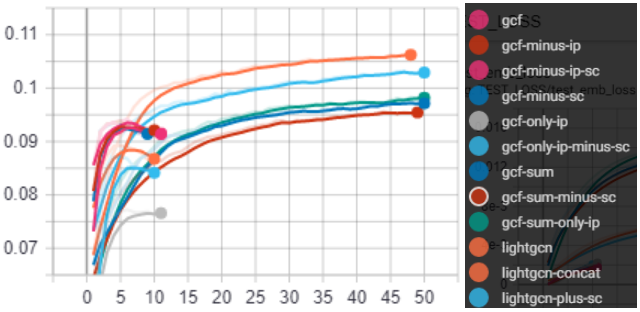
\includegraphics[width=\linewidth]{figures/gcf-all-ndcg.png}
    \caption{NDCG@50 for the Yelp2020 dataset.}
    \label{fig:GCF-NDCG-ablation-study}
\end{figure}
\begin{figure}[]
    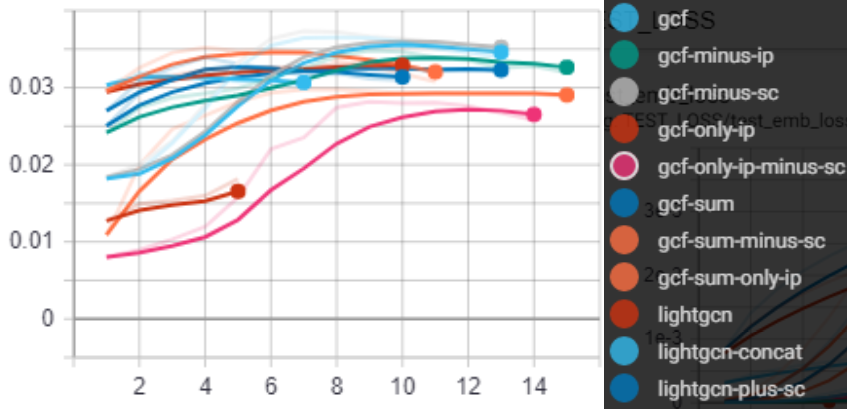
\includegraphics[width=\linewidth]{figures/amazon-cell-sport-gcf-all-ndcg.png}
    \caption{NDCG@50 for the Amazon-Sport-Cell dataset.}
    \label{fig:GCF-NDCG-ablation-study-amazon-cell-sport}
\end{figure}
\begin{figure}[]
    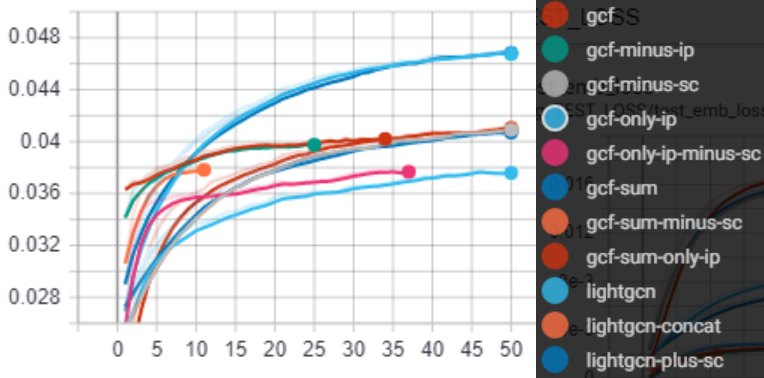
\includegraphics[width=\linewidth]{figures/amazon-book-gcf-all-ndcg.png}
    \caption{NDCG@50 for the Amazon-Book dataset.}
    \label{fig:GCF-NDCG-ablation-study-amazon-book}
\end{figure}

\subsubsection{Inner product}
Inner product makes methods using weighted summation perform worse most of the time.
The only exception is Recall@50 on Amazon-Cell-Sport for \textit{GCF-sum} which performs better than LightGCN.
This could also simply be because the inner product in general is beneficial for datasets where users or items have few connections.
For \textit{GCF} and \textit{GCF-minus-ip} it makes a small difference to add inner product in Yelp2020 and Amazon-Book, however for Amazon-Cell-Sport the method using inner product performs 3.8 \% better for Recall@50 and 6 \% better for NDCG@50.
These result can indicate that utilizing inner product is favorable when using smaller datasets.

\subsubsection{Self connections}
When comparing the counter parting methods on \autoref{tab:ablation-results} that either utilize or do not utilize self connections there is often a minimal difference on the results.
For LightGCN, GCF and GCF sum, the counterparting methods with or without self connections makes a small difference.
For \textit{LightGCN} and \textit{LightGCN-plus-sc} it varies which one performs best, but \textit{GCF-minus-sc} outperforms \textit{GCF} by a small amount most of the time.
Interestingly \textit{gcf-only-ip-minus-sc} performs significantly better than \textit{gcf-only-ip} on Yelp2020 and Amazon-Cell-Sport, which can indicate that self connections are harmful for performance, if you only use inner product in the convolutions.
However on Amazon-Book it makes a small difference.

\subsubsection{Conclusion}
The best performing methods is either GCF or LightGCN with or without self connections.
GCF is the best performing on Amazon-Cell-Sport, which is the smallest datasets, that also includes a lot of items with very few interactions.
We assume that a combination of inner product and concatenation is beneficial for learning on small datasets.
But on the larger datasets, LightGCN and LightGCN-plus-sc is the best performing methods.
\subsection{Changing $\alpha_k$}

\subsubsection{Removing $\alpha_k$}\label{subsubsec:remove-alpha-k}
In this experiment we changed $\alpha_k$ from $(1 / (K + 1))$ to $1$ and essentially removed the variable to see what impact it had on the results.
This method is called LightGCN-Ak1 which stands for LightGCN $\alpha_k = 1$.
This will result in the embeddings scaling more than they otherwise would have with $\alpha_k$ as normalization.
As can be seen on \autoref{fig:ndcg-yelp2020-alpha-k} and \autoref{fig:recall-yelp2020-alpha-k} changing $\alpha_k$ decreases performance of LightGCN on the yelp2020 dataset.
In the initial epochs, LightGCN-Ak1 performs better, but quickly starts to decline in performance.
On \autoref{fig:ndcg-amazon-alpha-k} and \autoref{fig:recall-amazon-alpha-k} LightGCN and LightGCN-Ak1 was run on the amazon-book dataset, but can seen that LightGCN still outperforms LightGCN-Ak1.
These results indicates that $\alpha_k$ is an important part of the layer combination for weighted summation, and we will continue our experimentation on trying to optimize $\alpha_k$
\begin{figure}
    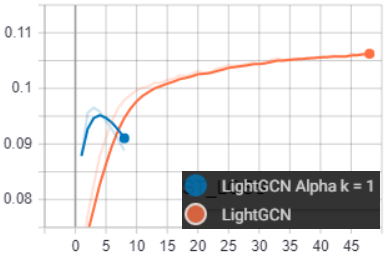
\includegraphics[width=\linewidth]{figures/alpha-k-results/yelp2020-ndcg.png}
    \caption{NDCG@50 of LightGCN and LightGCN-Ak1 on yelp2020}
    \label{fig:ndcg-yelp2020-alpha-k}
\end{figure}
\begin{figure}
    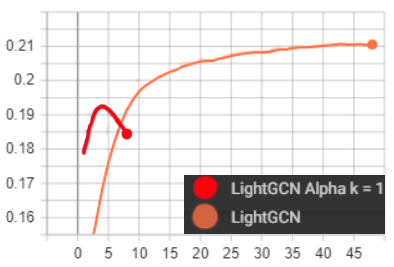
\includegraphics[width=\linewidth]{figures/alpha-k-results/yelp2020-recall.png}
    \caption{Recall@50 of LightGCN and LightGCN-Ak1 on yelp2020}
    \label{fig:recall-yelp2020-alpha-k}
\end{figure}
\begin{figure}
    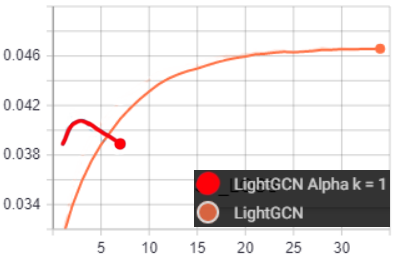
\includegraphics[width=\linewidth]{figures/alpha-k-results/amazon-ndcg.png}
    \caption{NDCG@50 of LightGCN and LightGCN-Ak1 on amazon-book}
    \label{fig:ndcg-amazon-alpha-k}
\end{figure}
\begin{figure}
    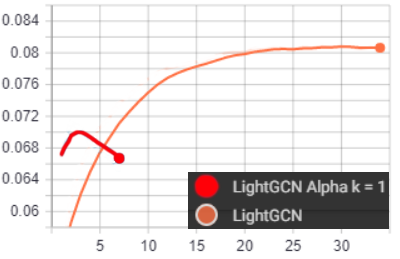
\includegraphics[width=\linewidth]{figures/alpha-k-results/amazon-recall.png}
    \caption{Recall@50 of LightGCN and LightGCN-Ak1 on amazon-book}
    \label{fig:recall-amazon-alpha-k}
\end{figure}

\subsubsection{Utilizing only one layer}
We showed previously that removing $\alpha_k$ was harmful for the performance. 
Therefore we want to investigate what influence the different layers have on the performance.
In this section we experiment with removing the layer combination, and only utilizing a specific convolution layers.
$\mathbf{e}^{(0)}$, $\mathbf{e}^{(1)}$, $\mathbf{e}^{(2)}$, $\mathbf{e}^{(3)}$, $\mathbf{e}^{(4)}$ and $\mathbf{e}^{(5)}$ are used as the final embeddings in each experiment respectively.
These are compared to LightGCN where weighted sum is utilized with a different number of layers.
\begin{table*}[]
    \centering
    \begin{tabular}{|l|l|l|l|l|l|l|}
        \hline
                             & \multicolumn{2}{l|}{Amazon-Cell-Sport} & \multicolumn{2}{l|}{Yelp2020} & \multicolumn{2}{l|}{Amazon-Book}                                                                 \\ \hline
                             & NDCG@50                                & Recall@50                     & NDCG@50                          & Recall@50         & NDCG@50             & Recall@50           \\ \hline
        Weighted sum (1 con) & 0.02804                                & 0.05503                       & 0.0969                           & 0.1955            & 0.0427              & 0.07408             \\ \hline
        Weighted sum (2 con) & 0.03132                                & 0.06133                       & 0.1008                           & 0.2015            & 0.0463              & 0.08055             \\ \hline
        Weighted sum (3 con) & 0.03237                                & 0.06447                       & 0.1064                           & 0.2106            & \textbf{0.04668}    & \textbf{0.08129}    \\ \hline
        Weighted sum (4 con) & 0.03253                                & 0.06394                       & 0.1084                           & 0.2157            & \underline{0.04617} & \underline{0.08033} \\ \hline
        Weighted sum (5 con) & 0.03285                                & 0.06451                       & \textbf{0.1089}                  & \textbf{0.2177}   & 0.04515             & 0.07861             \\ \hline
        $\mathbf{e}^{(0)}$   & 0.02169                                & 0.04447                       & 0.08177                          & 0.1674            & 0.03669             & 0.06373             \\ \hline
        $\mathbf{e}^{(1)}$   & 0.02523                                & 0.04859                       & 0.1019                           & 0.2039            & 0.0458              & 0.079               \\ \hline
        $\mathbf{e}^{(2)}$   & 0.03419                                & 0.06809                       & \underline{0.1086}               & \underline{0.217} & 0.04487             & 0.07755             \\ \hline
        $\mathbf{e}^{(3)}$   & 0.03483                                & 0.06972                       & 0.09956                          & 0.2001            & 0.0372              & 0.06412             \\ \hline
        $\mathbf{e}^{(4)}$   & \underline{0.0366}                     & \textbf{0.07377}              & 0.08863                          & 0.1788            & 0.03247             & 0.05607             \\ \hline
        $\mathbf{e}^{(5)}$   & \textbf{0.03733}                       & \underline{0.07318}           & 0.0819                           & 0.1643            & 0.02923             & 0.05022             \\ \hline
    \end{tabular}
    \centering
    \caption{Experiment on LightGCN where different layers are used as the final embedding compared with weighted sum.}
    \label{tab:only-use-one-layer-experiment}
\end{table*}

As can be seen on \autoref{tab:only-use-one-layer-experiment} the results vary a lot depending on the dataset.
For Amazon-Cell-Sport only considering $e^{(4)}$ and $e^{(5)}$ gives the best results which perform around 13 \% better than weighted sum with 5 convolutions.
This could be because Amazon-Cell-Sport consists of many nodes with few interactions, and therefore the later convolutions have the largest impact. 90 \% of all items within this dataset have 5 interactions, which is one of the reasons that the later convolutions perform so well.
For Yelp2020 the best results were weighted sum with 5 convolutions closely followed by $e^{(2)}$.
This dataset varies more in terms of the number of interactions that the users have.
For Amazon-Book weighted sum with 3 convolutions performs best and this could be because there is a large variation of how many interactions the users have.
One of the advantages of weighted sum is that it stabilizes the results.
This might have a positive effect in some cases compared to our method where we only use the embedding from one of the layers.
The difference on the results of weighted sum is in each dataset not that different compared to using one embedding layer.

%\subsection{Adjusted layer combination}\label{subsec:adjusted-layer-combination}
One suggestion made by LightGCN was to personalize the layer combination, so that sparse users could benefit more from higher-order neighbors \cite{lightgcn}.
The results seen in \autoref{subsec:degree-experiment} indicate that there are is no direct correlation between the degree of a node and the nodes performance.
In this experiment we used the results from \autoref{subsec:degree-experiment} to calculate the layer effects by using the algorithms described in \autoref{fredsplit}.
All of the nodes will have the same calculated layer effects because we used the overall performance of the nodes to calculate them and not the individual performance of each node degree range.

\subsubsection{Degree depending layer combination}
% Skal omskrives når vi har indsat resultaterne i appendix
The results from this experiment can be seen in Appendix \ref{app:adjusted-layer-combi}.
Results needs to be described when they are finished.

\subsubsection{Balanced Layer Combination}
The experiments conducted using the balanced method described in \autoref{fredsplit} are described in this section.
It was calculated from the NDCG@50 results on each layer, seen on \autoref{tab:yelp2020-ndcg-evaluation}, \autoref{tab:amazon-book-NDCG-evaluation} and \autoref{tab:Amazon-Cell-Sport-ndcg-evaluation}.
The splits in the following itemize were calculated from this method.
\begin{table*}[]
    \centering
    \begin{tabular}{|l|r|r|r|r|r|r|}
        \hline
                          & $\mathbf{E}^{(0)}$ & $\mathbf{E}^{(1)}$ & $\mathbf{E}^{(2)}$ & $\mathbf{E}^{(3)}$ & $\mathbf{E}^{(4)}$ & $\mathbf{E}^{(5)}$ \\ \hline
        Amazon-Cell-Sport & 0.07412            & 0.03412            & 0.17319            & 0.19376            & 0.25066            & 0.27412            \\ \hline
        Yelp2020          & 0.10576            & 0.23173            & 0.30576            & 0.20587            & 0.08510            & 0.06576            \\ \hline
        Amazon-Book       & 0.12045            & 0.38566            & 0.35858            & 0.13529            &                    &                    \\ \hline
    \end{tabular}
    \caption{Layer effects for the different datasets for the balanced method..}
    \label{tab:layer-effect}
\end{table*}

The results from this experiment can be seen in \autoref{tab:balanced-layer-effect}.
Generally it can be observed that the results vary depending on the dataset.
For Amazon-Cell-Sport improves with 7.03 \% using this method.
This is a substantial improvement compared to the results from Yelp2020 and Amazon-Book.
However, for Amazon-Cell-Sport only utilizing $\mathbf{e^{(4)}}$ or $\mathbf{e^{(5)}}$ as seen on \autoref{tab:only-use-one-layer-experiment} is an better alternative.
For Yelp2020 there is a small improvement of 1.15 \% in NDCG and 0.68 \% in Recall.
For Amazon-Book there is a decrease in performance by -2.36 \% in NDCG and an improvement of 0.78 \% in recall.

\begin{table*}[h!]
    \centering
    \begin{tabular}{|l|r|r|r||l|r|r||l|l|l|}
        \hline
                  & \multicolumn{3}{c||}{Amazon-Cell-Sport} & \multicolumn{3}{c||}{Yelp2020} & \multicolumn{3}{c|}{Amazon-Book}                                                                                                                                              \\ \hline
                  & \multicolumn{1}{l|}{5 con}              & \multicolumn{1}{l|}{BLC}       & \multicolumn{1}{l||}{impr}            & 5 con  & \multicolumn{1}{l|}{BLC} & \multicolumn{1}{l||}{impr}            & 3 con   & BLC     & impr                                  \\ \hline
        NDCG@50   & 0.03285                                 & 0.03516                        & \textbf{\textcolor{OliveGreen}{7.03}} & 0.1089 & 0.11015                  & \textbf{\textcolor{OliveGreen}{1.15}} & 0.04647 & 0.04537 & \textbf{\textcolor{Maroon}{-2.36}}    \\ \hline
        Recall@50 & 0.06451                                 & 0.06928                        & \textbf{\textcolor{OliveGreen}{7.39}} & 0.2177 & 0.21917                  & \textbf{\textcolor{OliveGreen}{0.68}} & 0,08129 & 0,08066 & \textbf{\textcolor{OliveGreen}{0.78}} \\ \hline
    \end{tabular}
    \caption{NDCG@50 and Recall@50 results for balanced layer combination, where it was not based on the node degree.}
    \label{tab:balanced-layer-effect}
\end{table*}

\paragraph{Aggressive Layer Combination}
The experiments conducted using the aggressive method described in \autoref{fredsplit} are described in this section
The splits were calculated from NDCG @50 and can be seen in \autoref{tab:aggressive-balanced-layer-effect}.
\begin{table*}[]
    \centering
    \begin{tabular}{|l|r|r|r|r|r|r|}
        \hline
                          & $\mathbf{E}^{(0)}$ & $\mathbf{E}^{(1)}$ & $\mathbf{E}^{(2)}$ & $\mathbf{E}^{(3)}$ & $\mathbf{E}^{(4)}$ & $\mathbf{E}^{(5)}$ \\ \hline
        Amazon-Cell-Sport & 0.0                & 0.0                & 0.1658853          & 0.2110679          & 0.291968           & 0.331078           \\ \hline
        Yelp2020          & 0.0                & 0.2912216          & 0.4146101          & 0.228054           & 0.0661141          & 0.0                \\ \hline
        Amazon-Book       & 0.051091           & 0.43049            & 0.38988            & 0.12852            &                    &                    \\ \hline
    \end{tabular}
    \caption{Layer effects for the different datasets based on ALC.}
    \label{tab:aggressive-balanced-layer-effect}
\end{table*}
The results can be seen in \autoref{tab:aggressive-layer-combination}.
For Amazon-Cell-Sport it performed 8.37 \% better in NDCG and 8.54 \% better in recall than 5 convolution average.
This is a larger performance increase than BLC.
For Yelp2020 there is a small increase in performance with 0.57 \% in NDCG and 0.17 \% in Recall.
Here the BLC method had a larger improvement.
For Amazon-Book the decrease in performance for NDCG is smaller than for BLC by -1.57 \% and has an increase in recall by  2.65 \%.
\begin{table*}[h!]
    \centering
    \begin{tabular}{|l|r|r|r||l|r|r||l|l|l|}
        \hline
                  & \multicolumn{3}{c||}{Amazon-Cell-Sport} & \multicolumn{3}{c||}{Yelp2020} & \multicolumn{3}{c|}{Amazon-Book}                                                                                                                                                                  \\ \hline
                  & \multicolumn{1}{l|}{5 con}              & \multicolumn{1}{l|}{ALC}       & \multicolumn{1}{l||}{impr}            & \multicolumn{1}{l|}{5 con} & \multicolumn{1}{l|}{ALC} & \multicolumn{1}{l||}{impr}            & 3 con   & ALC     & impr                                  \\ \hline
        NDCG@50   & 0.03285                                 & 0.0356                         & \textbf{\textcolor{OliveGreen}{8.37}} & 0.1089                     & 0.10953                  & \textbf{\textcolor{OliveGreen}{0.57}} & 0.04647 & 0.04574 & \textbf{\textcolor{Maroon}{-1.57}}    \\ \hline
        Recall@50 & 0.06451                                 & 0.07002                        & \textbf{\textcolor{OliveGreen}{8.54}} & 0.2177                     & 0,.21809                 & \textbf{\textcolor{OliveGreen}{0.17}} & 0.08129 & 0.07919 & \textbf{\textcolor{OliveGreen}{2.65}} \\ \hline
    \end{tabular}
    \caption{NDCG@50 and Recall@50 results for aggressive layer combination, where it was not based on the node degree.}
    \label{tab:aggressive-layer-combination}
\end{table*}

\subsection{Conclusion on adjusted layer combination}
The results from these experiments show that our method is not an extension that would be beneficial for all datasets.
It does show a significant improvement, but this improvement is still smaller than the 13 \% improvement on Amazon-Cell-Sport by only taking $e^{(5)}$ into account.

\subsection{Performance Comparison with State-of-the-Arts}
In the following subsection experiments are conducted to answer the following research question:
\begin{itemize}
    \item \textbf{RQ3}: How does adding ALC and BLC to LightGCN perform compared to other state of the art methods?
\end{itemize}
\autoref{tab:baselines-ndcg} and \autoref{tab:baselines-recall} shows the results of our experiments with NDCG@50 and Recall@50 respectively.
We compare our method to LightGCN, NGCF, GC-MC and GCN.
All experiments were done with 5 convolutions. 
Amazon-Book actually performed better with 3 convolutions, but because ALC and BLC were calculated using 5 convolutions we decided to compare it with amazon-book using 5 convolutions.
ALC and BLC could possibly perform better on Amazon-Book with fewer convolutions.
The primary observations from the experiments are:
\begin{itemize}
    \item ALC, BLC and $\mathbf{e}^{(i)}$ generally perform better than all other methods, except for on Amazon-Cell-Electronic and Amazon-Cloth-Sport. Amazon-Cell-Electronic differentiates from other datasets because it has an item/user ratio of 17.42, while other datasets have an item/user ratio below 8. Amazon-Cloth-Sport is similar to Amazon-Cell-Sport in terms of item/user ratio, however, it has twice as many users and items.
    \item ALC and $\mathbf{e}^{(i)}$ often perform better than BLC in NDCG@50, but BLC often performs better than ALC in Recall@50. For NDCG@50 $\mathbf{e}^{(i)}$ seems to either be best performing or close to performing best in most of the cases, except for on Amazon-Cloth-Sport.
    \item LightGCN outperforms all other baseline methods, except for GCF in Amazon-Cell-Sport. We seem to be unable to reconstruct that GCF outperforms LightGCN consistently as seen in their paper BiTGCF \cite{BiTGCF}. This could be because BiTGCF uses cross-entropy as their loss function for all methods while we use BPR. Another reason could be because they utilize the evaluation protocol of "Leave-one-out" and LightGCN uses "All-Ranking" protocol \cite{BiTGCF,lightgcn}. GCF consistently outperforms NGCF and NGCF outperforms GCN and GC-MC most of the time. Between GCN and GC-MC it differs on the best performing depending on the dataset.
    \item We have not found any layer combination method that consistently can perform better than any other method. There is still work to be done to find a layer combination method that can combine the layers best suited for the datasets.
\end{itemize}
\begin{table*}[h!]
    \centering
    \begin{tabular}{|l|r|r|r|r|r||r|r|l|}
        \hline
        NDCG@50                 & \multicolumn{1}{l|}{NGCF} & \multicolumn{1}{l|}{LightGCN} & \multicolumn{1}{l|}{GCN} & \multicolumn{1}{l|}{GC-MC} & \multicolumn{1}{l||}{GCF} & \multicolumn{1}{l|}{ALC} & \multicolumn{1}{l|}{BLC} & $\mathbf{e}^{(i)}$      \\ \hline
        Yelp2020                & 0.08502                   & 0.1089                        & 0.07594                  & 0.07947                    & 0.09092                   & \underline{0.10953}      & \textbf{0.11015}         & 0.1086 (2)              \\ \hline
        Amazon-Book             & 0.03811                   & 0.04515                       & 0.03268                  & 0.03364                    & 0.04032                   & \underline{0.04574}      & 0.04537                  & \textbf{0.0458} (1)     \\ \hline
        Amazon-Cell-Sport       & 0.02476                   & 0.033                         & 0.02087                  & 0.01709                    & 0.03398                   & \underline{0.0356}       & 0.03516                  & \textbf{0.03733} (5)    \\ \hline
        Amazon-Cloth-Sport      & 0.05826                   & \underline{0.06749}           & 0.00996                  & 0.01074                    & \textbf{0.07556}          & 0.05945                  & 0.06356                  & 0.06392 (2)             \\ \hline
        Amazon-Cell-Electronic  & 0.03399                   & 0.05413                       & 0.02589                  & 0.0180                     & \textbf{0.05424}          & 0.05094                  & 0.05399                  & \underline{0.05422} (3) \\ \hline
        Amazon-Cloth-Electronic & 0.00912                   & 0.01710                       & 0.01384                  & 0.00829                    & 0.01272                   & \underline{0.01941}      & 0.01792                  & \textbf{0.02074} (5)    \\ \hline
    \end{tabular}
    \caption{Performance comparison on NDCG@50 with different state of the art methods.}
    \label{tab:baselines-ndcg}
\end{table*}

\begin{table*}[h!]
    \centering
    \begin{tabular}{|l|r|r|r|r|r||r|r|l|}
        \hline
        Recall@50               & \multicolumn{1}{l|}{NGCF} & \multicolumn{1}{l|}{LightGCN} & \multicolumn{1}{l|}{GCN} & \multicolumn{1}{l|}{GC-MC} & \multicolumn{1}{l||}{GCF} & \multicolumn{1}{l|}{ALC} & \multicolumn{1}{l|}{BLC} & $\mathbf{e}^{(i)}$      \\ \hline
        Yelp2020                & 0.17535                   & 0.2177                        & 0.15317                  & 0.16341                    & 0.1869                    & \underline{0.21809}      & \textbf{0.21917}         & 0.217 (2)               \\ \hline
        Amazon-Book             & 0.06714                   & 0.07861                       & 0.05578                  & 0.05826                    & 0.07035                   & \underline{0.07919}      & \textbf{0.08066}         & 0.079 (1)               \\ \hline
        Amazon-Cell-Sport       & 0.05312                   & 0.06451                       & 0.04119                  & 0.03723                    & 0.06536                   & \underline{0.07002}      & 0.06928                  & \textbf{0.07377} (4)    \\ \hline
        Amazon-Cloth-Sport      & 0.08501                   & 0.10482                       & 0.02070                  & 0.02817                    & 0.10385                   & 0.10240                  & \textbf{0.10567}         & \underline{0.10541} (2) \\ \hline
        Amazon-Cell-Electronic  & 0.05248                   & 0.07738                       & 0.03668                  & 0.02633                    & 0.07165                   & 0.07355                  & \underline{0.07846}      & \textbf{0.07909} (3)    \\ \hline
        Amazon-Cloth-Electronic & 0.01863                   & 0.03225                       & 0.02575                  & 0.01690                    & 0.02948                   & \underline{0.03760}      & 0.03506                  & \textbf{0.04061} (5)    \\ \hline
    \end{tabular}
    \caption{Performance comparison on Recall@50 with different state of the art methods.}
    \label{tab:baselines-recall}
\end{table*}

\subsection{Node degree experiment}\label{subsec:degree-experiment}
In this experiment we investigated how the nodes within a certain range of node degree perform. 
The node degree is the number of connections the node has in the original interaction graph.
Our initial hypothesis was that the fewer connections a node had, the more it would benefit from a higher number of convolutions.
However the results obviously confirm that this is not the case.
The NDCG results can be seen for Amazon-Cell-Sport on \autoref{tab:Amazon-Cell-Sport-ndcg-evaluation} and \autoref{fig:ndcg-individual-evaluation-amazon-book}, Yelp2020 on \autoref{tab:yelp2020-ndcg-evaluation} and \autoref{fig:yelp2020-ndcg-individual-evaluation} and Amazon-Book on \autoref{tab:amazon-book-NDCG-evaluation} and \autoref{fig:amazon-cell-sport-individual-evaluation-ndcg}.
The results have been evaluated within a certain node degree, and "All nodes" is where all nodes have been evaluated together to get the overall performance.
The \textbf{bold} results are the best performing and the \underline{underlined} results are the second best performing.
The rightmost column is the result of the best performing original LightGCN method, that were run with 1 to 5 convolutions.
All of the results for NDCG and Recall can be found in Appendix \ref{app:average-lightgcn-results}.
The tables and figures containing the results of the recall performance for the different degree ranges can be found in Appendix \ref{app:individual-recall-degree-experiment}.
The experiments for Amazon-Cell-Sport dataset can be seen on \autoref{tab:Amazon-Cell-Sport-ndcg-evaluation}.
These results showcase that for nodes with less than 46 connections that $E^{(5)}$ is usually the best performing embedding and for nodes with more than 46 connections $E^{(5)}$ performs worse than other embeddings with a lower number of convolutions.
$E^{(5)}$ does however often perform second best for many node degree ranges.
It is also worth noting that $E^{(3)}$, $E^{(4)}$ and $E^{(5)}$ consistently outperform LightGCN with 5 convolutions.
This could be because that utilizing $E^{(0)}$ and $E^{(1)}$ is harmful for performance, because 91 \% of all items only have between 1-5 connections and therefore the embeddings need more convolution to capture the collaborative signals.
Looking at the yelp2020 and amazon-book datasets seen on \autoref{tab:yelp2020-ndcg-evaluation} and \autoref{tab:amazon-book-NDCG-evaluation} the results do not seem to be dependent on the degree of the nodes, as almost all node degree ranges either perform best or second best in $E^{(1)}$ and $E^{(2)}$.
In both of these datasets nodes have above 19 connections on average and therefore the amount of collaborative signals increase much faster for each node in the graph compared to amazon-cell-sport.
For Amazon-Cell-Sport the Recall performance increases for the nodes with a higher degree, however for Yelp2020 and Amazon-Book it instead decreases with a larger node degree.
This could be because the nodes with many connections get too much noise in Yelp2020 and Amazon-Book, but for Amazon-Cell-Sport there are many items with few connected users, and hereby it limits how much information users with many connections gain.
The best result for all nodes in Amazon-Book is 3 convolution with average.
$E^{(1)}$ and $E^{(2)}$ significantly outperform the other embedding layers.  
For Yelp2020 the 5 convolution average performs best, while the $E^{(1)}$, $E^{(2)}$ and $E^{(3)}$ embedding layer are the best individual performing layer.
For Amazon-Cell-Sport $E^{(2)}$, $E^{(3)}$, $E^{(4)}$ and $E^{(5)}$ outperform the 5 convolution average.
\\
From these results we see an opportunity to change the layer combination in different ways to investigate if this will improve the results.
One experiment is simply to remove $E^{(0)}$, as it is often performing quite poorly on all used datasets.
Another experiment to conduct is to use the three best embedding layers for each method.
The last method is to use \autoref{fredsplit} method to optimize the hyper parameters.
As no direct link between the number of connections a user has and its performance was found, it could be interesting to look further into the number of implicit connections a user has once the convolutions have been performed. 
The conclusion on the results are that the individual degree of a node has a smaller effect on the final result than we initially expected.

%[tanker:]
%[ignore de dårligst embeddings og kun tag de bedst performance med når man laver layer combination]
%[- frederik model og std model]
%[fjern 0 embeding]
%[undersøg om der er en bestemt mængde connections en user/item kan have der giver optimal prediction]
%[- ud fra dette kunne man holde op med at lave con's for en user når de når en hvis mængde connections for at undgå støj]
%[lav simpel model der tager avg connections og vælger en mængde lag der skal have størst inflydelse]
%[måske have flere dataset som vi kan teste på]

% Yelp2020 NDCG
\begin{table*}[]
    \centering
    \begin{tabular}{|l|l|l|l|l|l|l||l|}
        \hline
        Node degree & \multicolumn{1}{c|}{$E^{(0)}$} & \multicolumn{1}{c|}{$E^{(1)}$} & \multicolumn{1}{c|}{$E^{(2)}$} & \multicolumn{1}{c|}{$E^{(3)}$} & \multicolumn{1}{c|}{$E^{(4)}$} & \multicolumn{1}{c||}{$E^{(5)}$} & \multicolumn{1}{c|}{5 con} \\ \hline
        6-10        & 0.07550                        & \underline{0.09271}            & 0.09136                        & 0.09211                        & 0.08228                        & 0.07408                         & \textbf{0.10095}           \\ \hline
        11-15       & 0.07677                        & \underline{0.09607}            & 0.09444                        & 0.09531                        & 0.08449                        & 0.07642                         & \textbf{0.10408}           \\ \hline
        16-20       & 0.08704                        & \underline{0.1069}             & 0.10575                        & 0.1043                         & 0.09354                        & 0.08562                         & \textbf{0.11451}           \\ \hline
        21-25       & 0.09096                        & \underline{0.1104}             & 0.10892                        & 0.1066                         & 0.09455                        & 0.08720                         & \textbf{0.11790}           \\ \hline
        26-30       & 0.08578                        & \underline{0.1137}             & 0.10933                        & 0.1092                         & 0.1000                         & 0.09431                         & \textbf{0.11909}           \\ \hline
        31-35       & 0.09420                        & 0.1196                         & \underline{0.12151}            & 0.1151                         & 0.1021                         & 0.09489                         & \textbf{0.12833}           \\ \hline
        36-40       & 0.09886                        & \underline{0.1195}             & 0.11764                        & 0.1108                         & 0.09965                        & 0.09326                         & \textbf{0.12711}           \\ \hline
        41-45       & 0.09512                        & 0.1071                         & \underline{0.11056}            & 0.1049                         & 0.09713                        & 0.09181                         & \textbf{0.11638}           \\ \hline
        46-50       & 0.09113                        & \underline{0.1162}             & 0.11447                        & 0.1147                         & 0.1057                         & 0.1011                          & \textbf{0.12537}           \\ \hline
        51-60       & 0.09782                        & 0.1095                         & \underline{0.11560}            & 0.1128                         & 0.1059                         & 0.1048                          & \textbf{0.12459}           \\ \hline
        61-70       & 0.09618                        & 0.1133                         & \underline{0.11338}            & 0.1125                         & 0.1024                         & 0.09921                         & \textbf{0.12377}           \\ \hline
        71-80       & 0.1067                         & \underline{0.1251}             & 0.12072                        & 0.1145                         & 0.1096                         & 0.1067                          & \textbf{0.13007}           \\ \hline
        81-90       & 0.09104                        & 0.1019                         & \underline{0.10477}            & 0.09683                        & 0.09489                        & 0.09547                         & \textbf{0.11042}           \\ \hline
        91-100      & 0.1045                         & \underline{0.1334}             & 0.13189                        & 0.1303                         & 0.1177                         & 0.1157                          & \textbf{0.14010}           \\ \hline
        101-150     & 0.09488                        & 0.1168                         & \underline{0.11731}            & 0.1142                         & 0.1077                         & 0.1092                          & \textbf{0.12676}           \\ \hline
        151-200     & 0.08451                        & 0.1066                         & \underline{0.11441}            & 0.1117                         & 0.1065                         & 0.1133                          & \textbf{0.11889}           \\ \hline
        201-250     & \textbf{0.1231}                & \underline{0.1217}             & 0.11866                        & 0.1009                         & 0.09105                        & 0.09490                         & \textbf{0.11999}           \\ \hline
        251-300     & 0.2238                         & 0.2224                         & 0.17787                        & 0.2538                         & 0.2806                         & \textbf{0.2917}                 & 0.21693                    \\ \hline
        301+        & 0.1752                         & 0.1989                         & \underline{0.21585}            & 0.2093                         & 0.1719                         & 0.1880                          & \textbf{0.23305}           \\ \hline
        All nodes   & 0.08177                        & 0.1019                         & \underline{0.1086}                         & 0.09956                        & 0.08863                        & 0.0819                          & \textbf{0.1089}            \\ \hline
    \end{tabular}
    \caption{NDCG@50 for Yelp2020 where only one convolution layer is used and compared with the best performing LightGCN convolution for Yelp2020.}
    \label{tab:yelp2020-ndcg-evaluation}
\end{table*}

\begin{figure}[]
    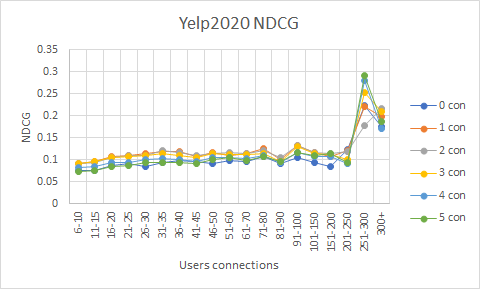
\includegraphics[width=0.5\textwidth]{figures/evaluation/yelp-ndcg-evaluation.png}
    \centering
    \caption{NDCG performance for the individual embedding layers on Yelp2020}
    \label{fig:yelp2020-ndcg-individual-evaluation}
\end{figure}

% Amazon-book
\begin{table*}[]
    \centering
    \begin{tabular}{|l|l|l|l|l|l|l||l|}
        \hline
        Node degree & \multicolumn{1}{c|}{$E^{(0)}$} & \multicolumn{1}{c|}{$E^{(1)}$} & \multicolumn{1}{c|}{$E^{(2)}$} & \multicolumn{1}{c|}{$E^{(3)}$} & \multicolumn{1}{c|}{$E^{(4)}$} & \multicolumn{1}{c|}{$E^{(5)}$} & \multicolumn{1}{c|}{3 con} \\ \hline
        16-20       & 0.03965                        & \underline{0.04851}            & 0.04722                        & 0.03762                        & 0.03287                        & 0.02911                        & \textbf{0.04929}           \\ \hline
        21-25       & 0.03903                        & \textbf{0.04862}               & 0.04807                        & 0.03788                        & 0.03323                        & 0.02964                        & \underline{0.04831}        \\ \hline
        26-30       & 0.03767                        & \textbf{0.04751}               & 0.04624                        & 0.03755                        & 0.03335                        & 0.03014                        & \textbf{0.04778}           \\ \hline
        31-35       & 0.03772                        & \textbf{0.04873}               & 0.04728                        & 0.03865                        & 0.03434                        & 0.03163                        & \underline{0.04825}        \\ \hline
        36-40       & 0.03412                        & \textbf{0.04506}               & \underline{0.04495}            & 0.03730                        & 0.03227                        & 0.02911                        & 0.04493                    \\ \hline
        41-45       & 0.03597                        & \textbf{0.04391}               & 0.04282                        & 0.03607                        & 0.03218                        & 0.02916                        & \underline{0.04301}        \\ \hline
        46-50       & 0.03436                        & 0.04350                        & \textbf{0.04413}               & 0.03784                        & 0.03357                        & 0.03111                        & \underline{0.04368}        \\ \hline
        51-60       & 0.03273                        & \underline{0.04205}            & 0.04077                        & 0.03380                        & 0.02959                        & 0.02719                        & \textbf{0.04210}           \\ \hline
        61-70       & 0.03214                        & \textbf{0.04109}               & \underline{0.04054}            & 0.03401                        & 0.03117                        & 0.02972                        & 0.03972                    \\ \hline
        71-80       & 0.03135                        & \textbf{0.03986}               & \underline{0.03958}            & 0.03445                        & 0.03160                        & 0.02981                        & 0.03923                    \\ \hline
        81-90       & 0.02832                        & \underline{0.03567}            & \textbf{0.03624}               & 0.03140                        & 0.02928                        & 0.02747                        & 0.03551                    \\ \hline
        91-100      & 0.02885                        & \underline{0.03814}            & \textbf{0.03882}               & 0.03163                        & 0.02884                        & 0.02717                        & 0.03781                    \\ \hline
        101-150     & 0.02675                        & \textbf{0.03351}               & 0.03332                        & 0.02927                        & 0.02652                        & 0.02522                        & \underline{0.03334}        \\ \hline
        151-200     & 0.02594                        & \underline{0.03037}            & \textbf{0.03049}               & 0.02728                        & 0.02518                        & 0.02423                        & 0.02932                    \\ \hline
        201-250     & 0.02613                        & 0.03228                        & \textbf{0.03312}               & 0.03096                        & 0.02925                        & 0.02914                        & \underline{0.03242}        \\ \hline
        251-300     & 0.03153                        & \textbf{0.03682}               & 0.03492                        & 0.03594                        & 0.03508                        & 0.03581                        & \underline{0.03617}        \\ \hline
        301+        & 0.03219                        & 0.03874                        & \textbf{0.04227}               & 0.04137                        & 0.04169                        & \underline{0.04207}            & 0.04130                    \\ \hline
        All nodes     & 0.03669                        & \underline{0.0458}             & 0.04487                        & 0.0372                         & 0.03247                        & 0.02923                        & \textbf{0.04668}           \\ \hline
    \end{tabular}
    \caption{NDCG@50 for Amazon-Book}
    \label{tab:amazon-book-NDCG-evaluation}
\end{table*}
\begin{figure}[]
    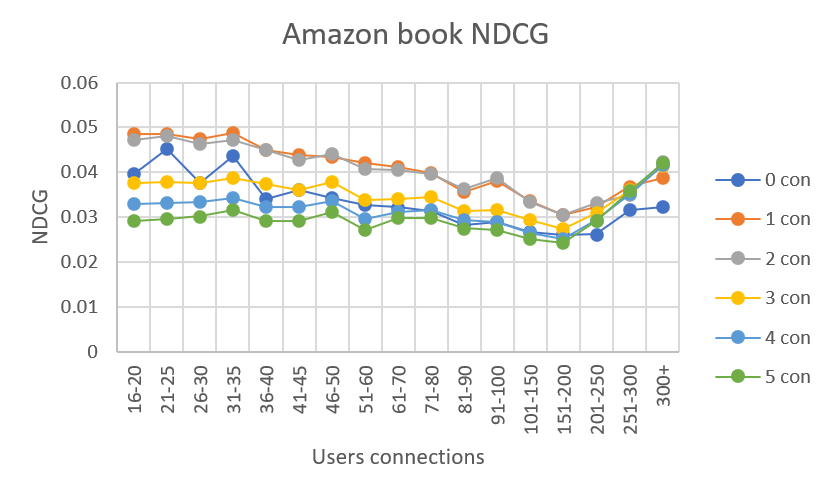
\includegraphics[width=0.5\textwidth]{figures/evaluation/amazon-book-ndcg.png}
    \centering
    \caption{NDCG performance for the individual embedding layers on Amazon-Book}
    \label{fig:ndcg-individual-evaluation-amazon-book}
\end{figure}

% Amazon-Cell-sport NDCG
\begin{table*}[]
    \centering
    \begin{tabular}{|l|l|l|l|l|l|l||l|}
        \hline
        Node degree & \multicolumn{1}{c|}{$E^{(0)}$} & \multicolumn{1}{c|}{$E^{(1)}$} & \multicolumn{1}{c|}{$E^{(2)}$} & \multicolumn{1}{c|}{$E^{(3)}$} & \multicolumn{1}{c|}{$E^{(4)}$} & \multicolumn{1}{c||}{$E^{(5)}$} & \multicolumn{1}{c|}{5 con} \\ \hline
        6-10        & 0.00995                        & 0.02156                        & 0.02250                        & 0.02173                        & \textbf{0.02441}               & \underline{0.02355}             & 0.01972                    \\ \hline
        11-15       & 0.01814                        & 0.02845                        & 0.02901                        & 0.02986                        & \underline{0.03154}            & \textbf{0.03376}                & 0.02984                    \\ \hline
        16-20       & 0.02378                        & 0.03269                        & 0.03737                        & \underline{0.03739}            & 0.03674                        & \textbf{0.03923}                & 0.03701                    \\ \hline
        21-25       & 0.03508                        & 0.04174                        & 0.04424                        & 0.04620                        & \underline{0.04727}            & \textbf{0.04907}                & 0.04438                    \\ \hline
        26-30       & 0.03584                        & 0.04281                        & 0.04606                        & 0.04663                        & \underline{0.04928}            & \textbf{0.04967}                & 0.04815                    \\ \hline
        31-35       & 0.05091                        & 0.06659                        & \textbf{0.07622}               & 0.06981                        & 0.07514                        & \underline{0.07544}             & 0.07514                    \\ \hline
        36-40       & 0.04884                        & 0.05221                        & \underline{0.06001}            & 0.05867                        & 0.05855                        & \textbf{0.06266}                & 0.05475                    \\ \hline
        41-45       & 0.6337                         & 0.07144                        & 0.07698                        & 0.07592                        & \underline{0.08052}            & \textbf{0.08197}                & 0.07634                    \\ \hline
        46-50       & 0.09049                        & 0.10755                        & \textbf{0.11442}               & 0.1030                         & 0.1067                         & \underline{0.1083}              & 0.10074                    \\ \hline
        51-60       & 0.05128                        & 0.07620                        & 0.08498                        & 0.09005                        & \textbf{0.1005}                & \underline{0.09309}             & 0.08827                    \\ \hline
        61-70       & 0.07796                        & 0.08878                        & 0.08324                        & 0.08425                        & \textbf{0.09537}               & \underline{0.09270}             & 0.07718                    \\ \hline
        71-80       & 0.04767                        & 0.05050                        & 0.05611                        & \textbf{0.05930}               & 0.05158                        & 0.05406                         & \underline{0.05834}        \\ \hline
        81-90       & 0.03265                        & 0.07549                        & 0.06440                        & 0.06200                        & \textbf{0.08332}               & \underline{0.08163}             & 0.07351                    \\ \hline
        91-100      & 0.06619                        & 0.07376                        & 0.07435                        & \textbf{0.09016}               & 0.08820                        & 0.08012                         & \underline{0.08968}        \\ \hline
        101-150     & 0.08542                        & 0.11063                        & \textbf{0.11732}               & 0.1151                         & 0.1130                         & \underline{0.1156}              & 0.11290                    \\ \hline
        151-200     & 0.07992                        & 0.08619                        & \textbf{0.10778}               & 0.08642                        & 0.09375                        & 0.08577                         & \underline{0.09668}        \\ \hline
        201-250     & 0.0                            & 0.0                            & 0.0                            & 0.0                            & 0.0                            & 0.0                             & 0.0                        \\ \hline
        251-300     & 0.0                            & 0.0                            & 0.0                            & 0.0                            & 0.0                            & 0.0                             & 0.0                        \\ \hline
        300+        & 0.11521                        & 0.16210                        & 0.12260                        & \underline{0.1752}             & \textbf{0.1786}                & 0.1680                          & 0.16771                    \\ \hline
        All nodes     & 0.02169                        & 0.02523                        & 0.03419                        & 0.03483                        & \underline{0.0366}             & \textbf{0.03733}                & 0.03285                    \\ \hline
    \end{tabular}
    \caption{NDCG@50 for Amazon-Cell-Sport where only one convolution layer is used.}
    \label{tab:Amazon-Cell-Sport-ndcg-evaluation}
\end{table*}
\begin{figure}[]
    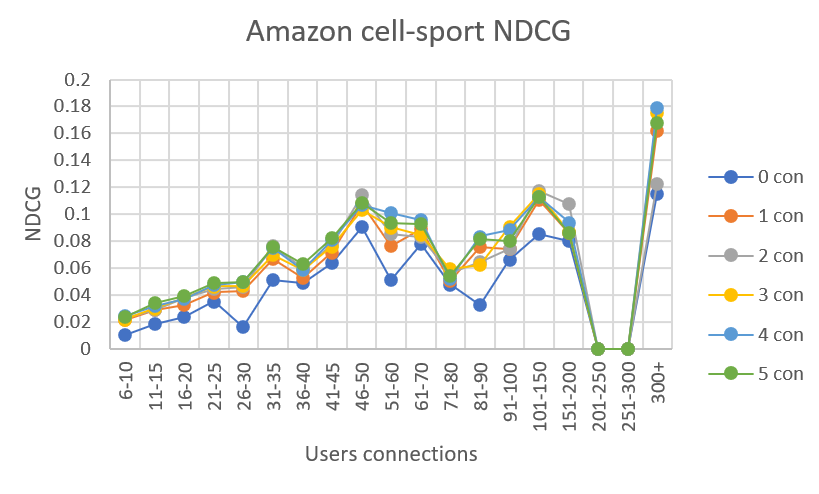
\includegraphics[width=0.5\textwidth]{figures/evaluation/amazon-cell-sport-ndcg.png}
    \centering
    \caption{NDCG performance for the individual embedding layers on Amazon-Cell-Sport}
    \label{fig:amazon-cell-sport-individual-evaluation-ndcg}
\end{figure}

